\documentclass[12pt]{article}
\usepackage[utf8]{inputenc}
\usepackage{booktabs}
\usepackage{graphicx}
\usepackage{amsmath}
\usepackage[margin=1in]{geometry}
\usepackage{setspace}
\doublespacing

\title{Physical Activity and Next-Day Mood Across the Menstrual Cycle: An Observational Study}
\author{}
\date{}

\begin{document}

\maketitle

% ============================================
% WHAT THIS PAPER ADDS (BMJ style box)
% ============================================
\begin{center}
\fbox{
\begin{minipage}{0.9\textwidth}
\textbf{What is already known on this topic}
\begin{itemize}
\item Physical activity is associated with improved mood and reduced risk of depression
\item Female sex hormones influence neurotransmitter systems involved in mood regulation
\item The menstrual cycle creates systematic within-person hormonal variation
\end{itemize}

\textbf{What this study adds}
\begin{itemize}
\item The association between physical activity and next-day mood varies substantially across menstrual cycle phases
\item The strongest mood benefit occurs during the follicular phase (7.6\% improvement), while no significant benefit was observed during the late luteal phase
\item Men showed no such phase variation, suggesting the effect in women is attributable to the menstrual cycle rather than calendar patterns
\end{itemize}
\end{minipage}
}
\end{center}

% ============================================
% INTRODUCTION - OUTLINE
% ============================================
\section*{Introduction}

% Paragraph 1: The Problem
% - Mental health burden globally, particularly depression/mood disorders
% - Physical activity established as protective factor for mental health
% - Growing interest in lifestyle interventions as accessible, low-cost strategies
% - However, effect sizes vary considerably across studies - why?

% Paragraph 2: What Is Known
% - Exercise acutely improves mood (meta-analyses)
% - Effects mediated by endorphins, BDNF, serotonin, dopamine
% - Women have higher rates of depression than men
% - Female sex hormones (oestrogen, progesterone) influence:
%   - Neurotransmitter systems
%   - Neuroplasticity
%   - Mood regulation
% - Menstrual cycle creates natural within-person hormonal variation

% Paragraph 3: The Gap
% - Most exercise-mood research ignores menstrual cycle
% - When cycle is considered, focus is usually on:
%   - Exercise performance, not mental health outcomes
%   - How mood affects exercise behaviour (not reverse)
% - Limited evidence on whether activity-mood relationship varies by cycle phase
% - If it does vary, this has implications for:
%   - Timing of interventions
%   - Personalised recommendations
%   - Understanding treatment heterogeneity

% Paragraph 4: Study Aims
% - Primary aim: Test whether the association between physical activity and next-day mood differs across menstrual cycle phases
% - Secondary aim: Use male control group with arbitrary calendar phases to rule out non-biological explanations
% - Hypotheses:
%   - Activity-mood association will vary by cycle phase in women
%   - No such variation expected in men (supporting biological mechanism)

% ============================================
% METHODS
% ============================================
\section*{Methods}

\subsection*{Study Design and Participants}

We conducted an observational study using prospectively collected data from a commercial health tracking application (Juli). The study analysed two independent samples: women who had recorded menstrual cycle data (n=138) and men serving as a control group (n=966). Women were eligible if they had recorded menstrual period start dates and had cycle lengths between 21 and 35 days. All participants were required to have recorded both physical activity and mood data on consecutive days.

\subsection*{Measures}

\subsubsection*{Menstrual Cycle Phase}

Cycle day was calculated relative to self-reported period start dates. Day 0 represented the first day of menstruation, with subsequent days numbered sequentially. Days preceding the next period were numbered backwards ($-$1 to $-$14), with negative numbering taking priority for overlapping dates. We defined four cycle phases based on established conventions: menstruation (days 0--5), follicular (days 6--13), early luteal (days $-$14 to $-$8), and late luteal (days $-$7 to $-$1).

\subsubsection*{Pseudo-Cycle Phase (Male Control Group)}

To determine whether any observed phase-specific effects in women could reflect general calendar patterns rather than menstrual cycle physiology, we created analogous pseudo-phases for men. The first Monday of each calendar month served as the anchor point (day 0), with subsequent days numbered 0--27. Phase intervals matched those used for women: Phase 1 (days 0--5), Phase 2 (days 6--13), Phase 3 (days 14--20), and Phase 4 (days 21--27).

\subsubsection*{Physical Activity}

Daily physical activity was quantified as activity minutes, calculated as (daily step count $\div$ 100) + workout duration in minutes. This conversion is based on the CADENCE-Adults study, which established that 100 steps per minute corresponds to moderate-intensity walking. Days were classified as active if activity minutes exceeded the participant's personal median, and inactive otherwise. This within-person median split ensured each individual served as their own control, accounting for individual differences in baseline activity levels.

\subsubsection*{Mood}

Mood was assessed daily using the application's mood score. The outcome variable was next-day mood, operationalised by aligning mood scores with the previous day's activity level. To account for individual differences in baseline mood, scores were normalised as percentage change from each participant's mean: ((score $-$ personal mean) $\div$ personal mean) $\times$ 100.

\subsection*{Statistical Analysis}

We used linear mixed-effects models with random intercepts for participants to account for the repeated-measures structure of the data. The primary model examined the interaction between activity status and cycle phase:

\begin{equation*}
\text{next-day mood} \sim \text{activity status} \times \text{cycle phase} + (1|\text{participant})
\end{equation*}

Phase-specific effects of activity were derived from the interaction model, with 95\% confidence intervals calculated using the delta method. We tested for heterogeneity in the activity-mood association across phases using a likelihood ratio test comparing models with and without the interaction term ($\chi^2$, 3 degrees of freedom).

For visualisation, daily means were smoothed using Fourier series with three harmonics to capture the periodic nature of the 28-day cycle while reducing noise.

Analyses were conducted in Python 3 using statsmodels for mixed-effects models and scipy for statistical tests. Statistical significance was set at $\alpha$=0.05.

\subsection*{Patient and Public Involvement}

Participants were not involved in setting the research question or outcome measures, nor were they involved in the design, recruitment, or conduct of the study. We plan to disseminate findings through the health application used for data collection.

% ============================================
% RESULTS
% ============================================
\section*{Results}

\subsection*{Participants}

The female sample comprised 138 women contributing 4151 person-days of observation. The male control sample comprised 966 men contributing 10,565 person-days (table 1). The within-person median split produced balanced comparison groups in both samples (women: 48.9\% inactive days, 51.1\% active days; men: 50.4\% inactive, 49.6\% active).

\subsection*{Physical Activity and Next-Day Mood in Women}

Days with above-median activity were associated with significantly better next-day mood (main effect: 1.61\% improvement, 95\% confidence interval 0.65\% to 2.57\%, P=0.001). This overall effect, however, masked substantial heterogeneity across cycle phases (likelihood ratio test: $\chi^2$=22.52, df=3, P$<$0.0001).

Table 2 presents phase-specific effects. The strongest association was observed during the follicular phase, when being active was associated with 7.6\% higher next-day mood compared with inactive days (95\% confidence interval 4.6\% to 10.7\%, P$<$0.001). Significant positive associations were also found during menstruation (3.5\%, 0.2\% to 6.8\%, P=0.036) and the early luteal phase (3.5\%, 0.1\% to 6.9\%, P=0.044). No significant association was observed during the late luteal phase (0.8\%, $-$2.6\% to 4.3\%, P=0.64).

Figure 1 displays these patterns graphically, showing smoothed mood trajectories for active versus inactive days across the cycle. The gap between active and inactive days varied markedly, peaking during the follicular phase and narrowing during the late luteal phase.

\subsection*{Male Control Analysis}

Men showed a modest overall association between activity and next-day mood (1.61\%, 95\% confidence interval 0.67\% to 2.55\%, P$<$0.001), similar in magnitude to the overall effect in women. In contrast to women, however, men showed no significant heterogeneity across pseudo-phases (likelihood ratio test: $\chi^2$=7.08, df=3, P=0.07).

Phase-specific effects in men were uniformly modest, ranging from 1.3\% to 2.0\% (table 2). Only Phase 2 (equivalent to the follicular period, days 6--13) reached statistical significance (2.0\%, 0.3\% to 3.8\%, P=0.02), though this effect was less than one third the magnitude of the corresponding follicular phase effect in women.

Figure 2 shows that in men the gap between active and inactive days remained relatively constant across all pseudo-phases, in marked contrast to the pattern observed in women.

\subsection*{Comparison of Effect Sizes}

The follicular phase effect in women (7.6\%) was 3.8 times larger than the equivalent phase effect in men (2.0\%). The difference between the strongest and weakest phase effects was 6.8 percentage points in women (follicular versus late luteal) compared with only 0.7 percentage points in men (Phase 2 versus Phase 3).

% ============================================
% FIGURE 1 PLACEHOLDER
% ============================================
\begin{figure}[htbp]
\centering
% 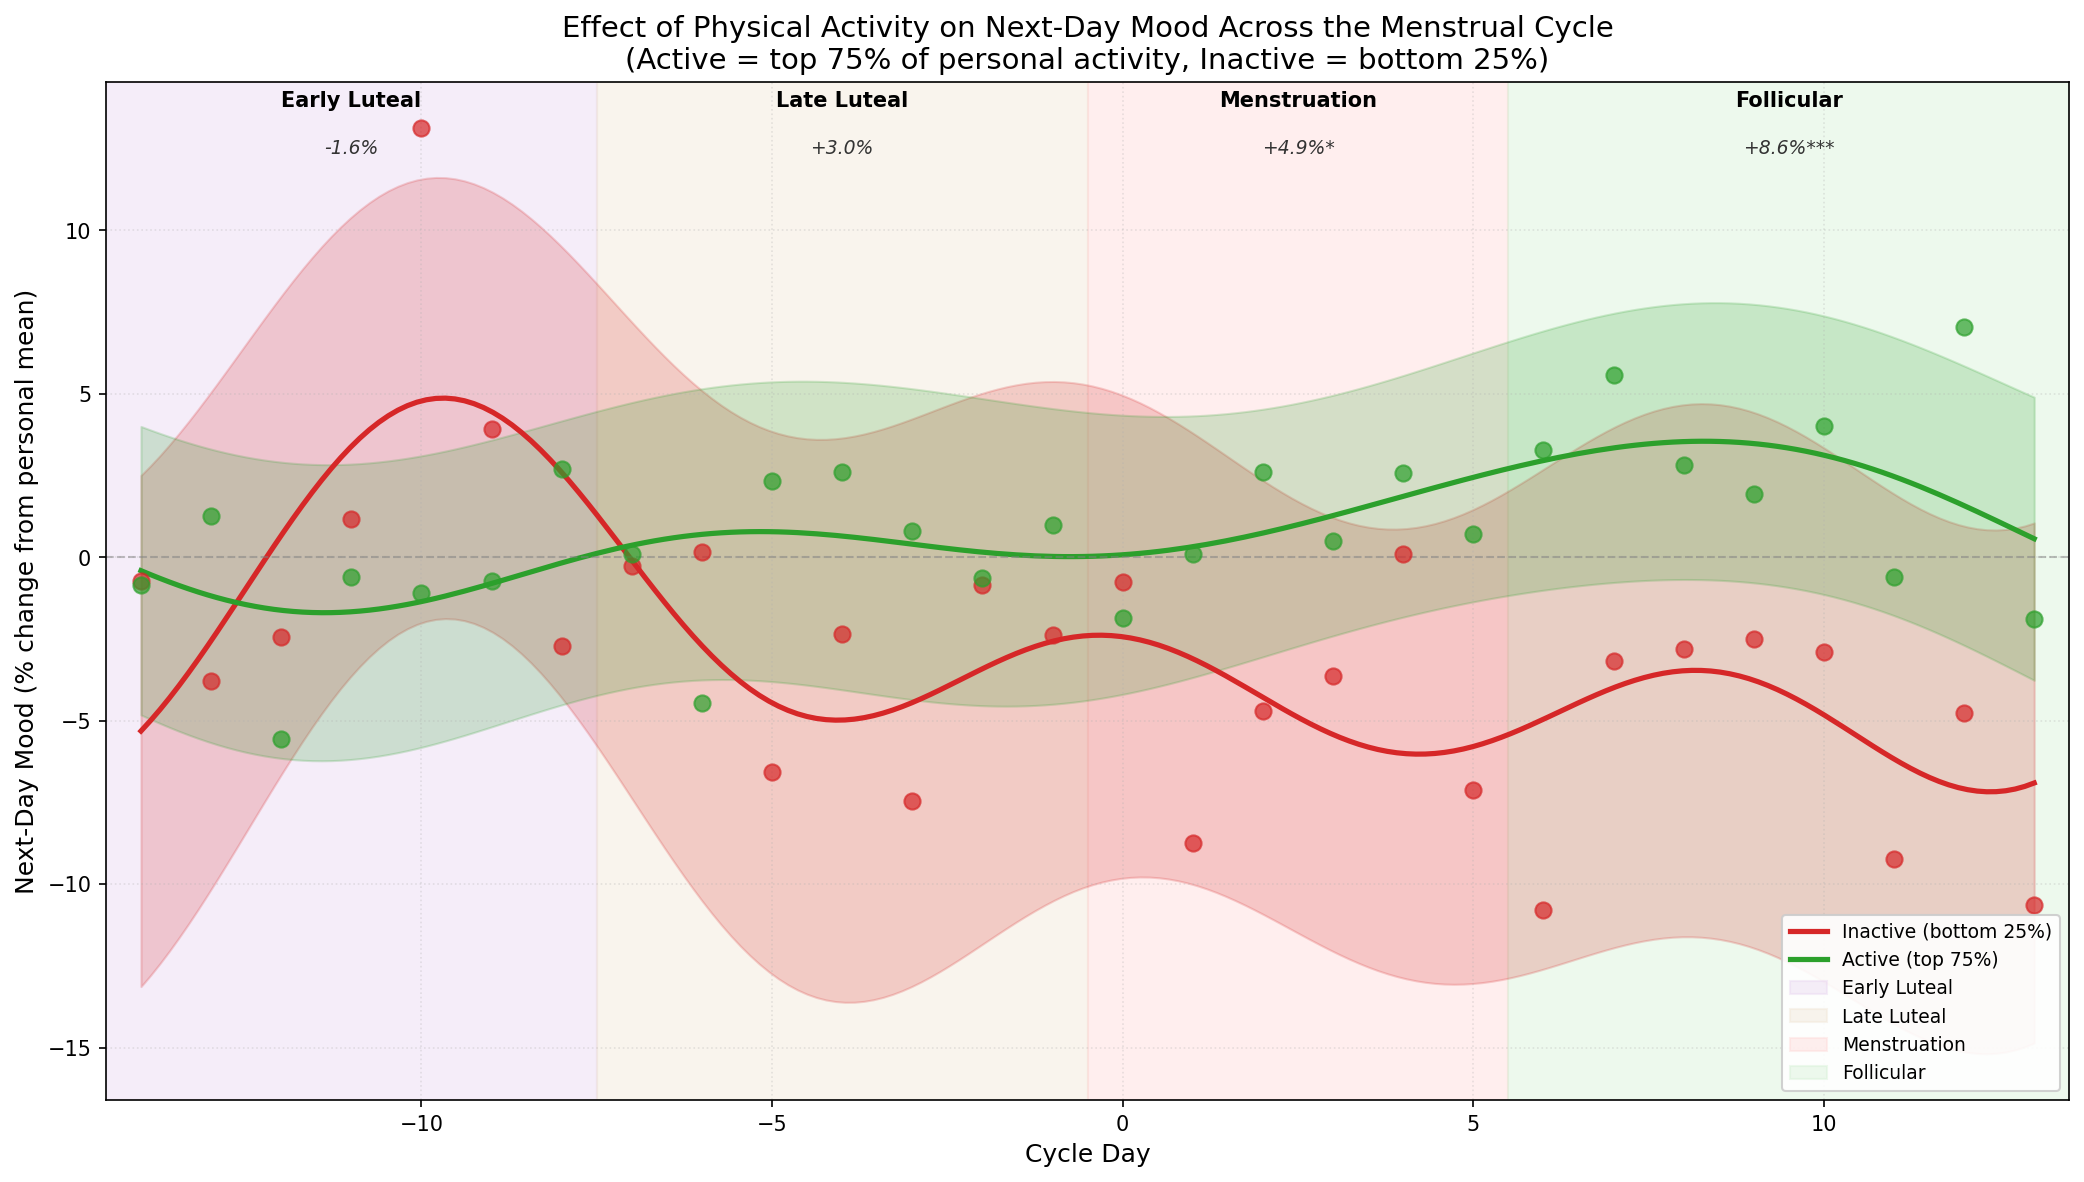
\includegraphics[width=\textwidth]{mood_by_cycle_day.png}
\fbox{\parbox{0.9\textwidth}{\centering\vspace{3cm}\textbf{Figure 1: Women}\\ Insert mood\_by\_cycle\_day.png\vspace{3cm}}}
\caption{Next-day mood by cycle day and activity status in women. Points represent daily means; lines show Fourier-smoothed trajectories with 90\% confidence bands. Background shading indicates cycle phases: menstruation (pink), follicular (green), early luteal (purple), and late luteal (tan). The gap between active and inactive days peaks during the follicular phase.}
\label{fig:women}
\end{figure}

% ============================================
% FIGURE 2 PLACEHOLDER
% ============================================
\begin{figure}[htbp]
\centering
% 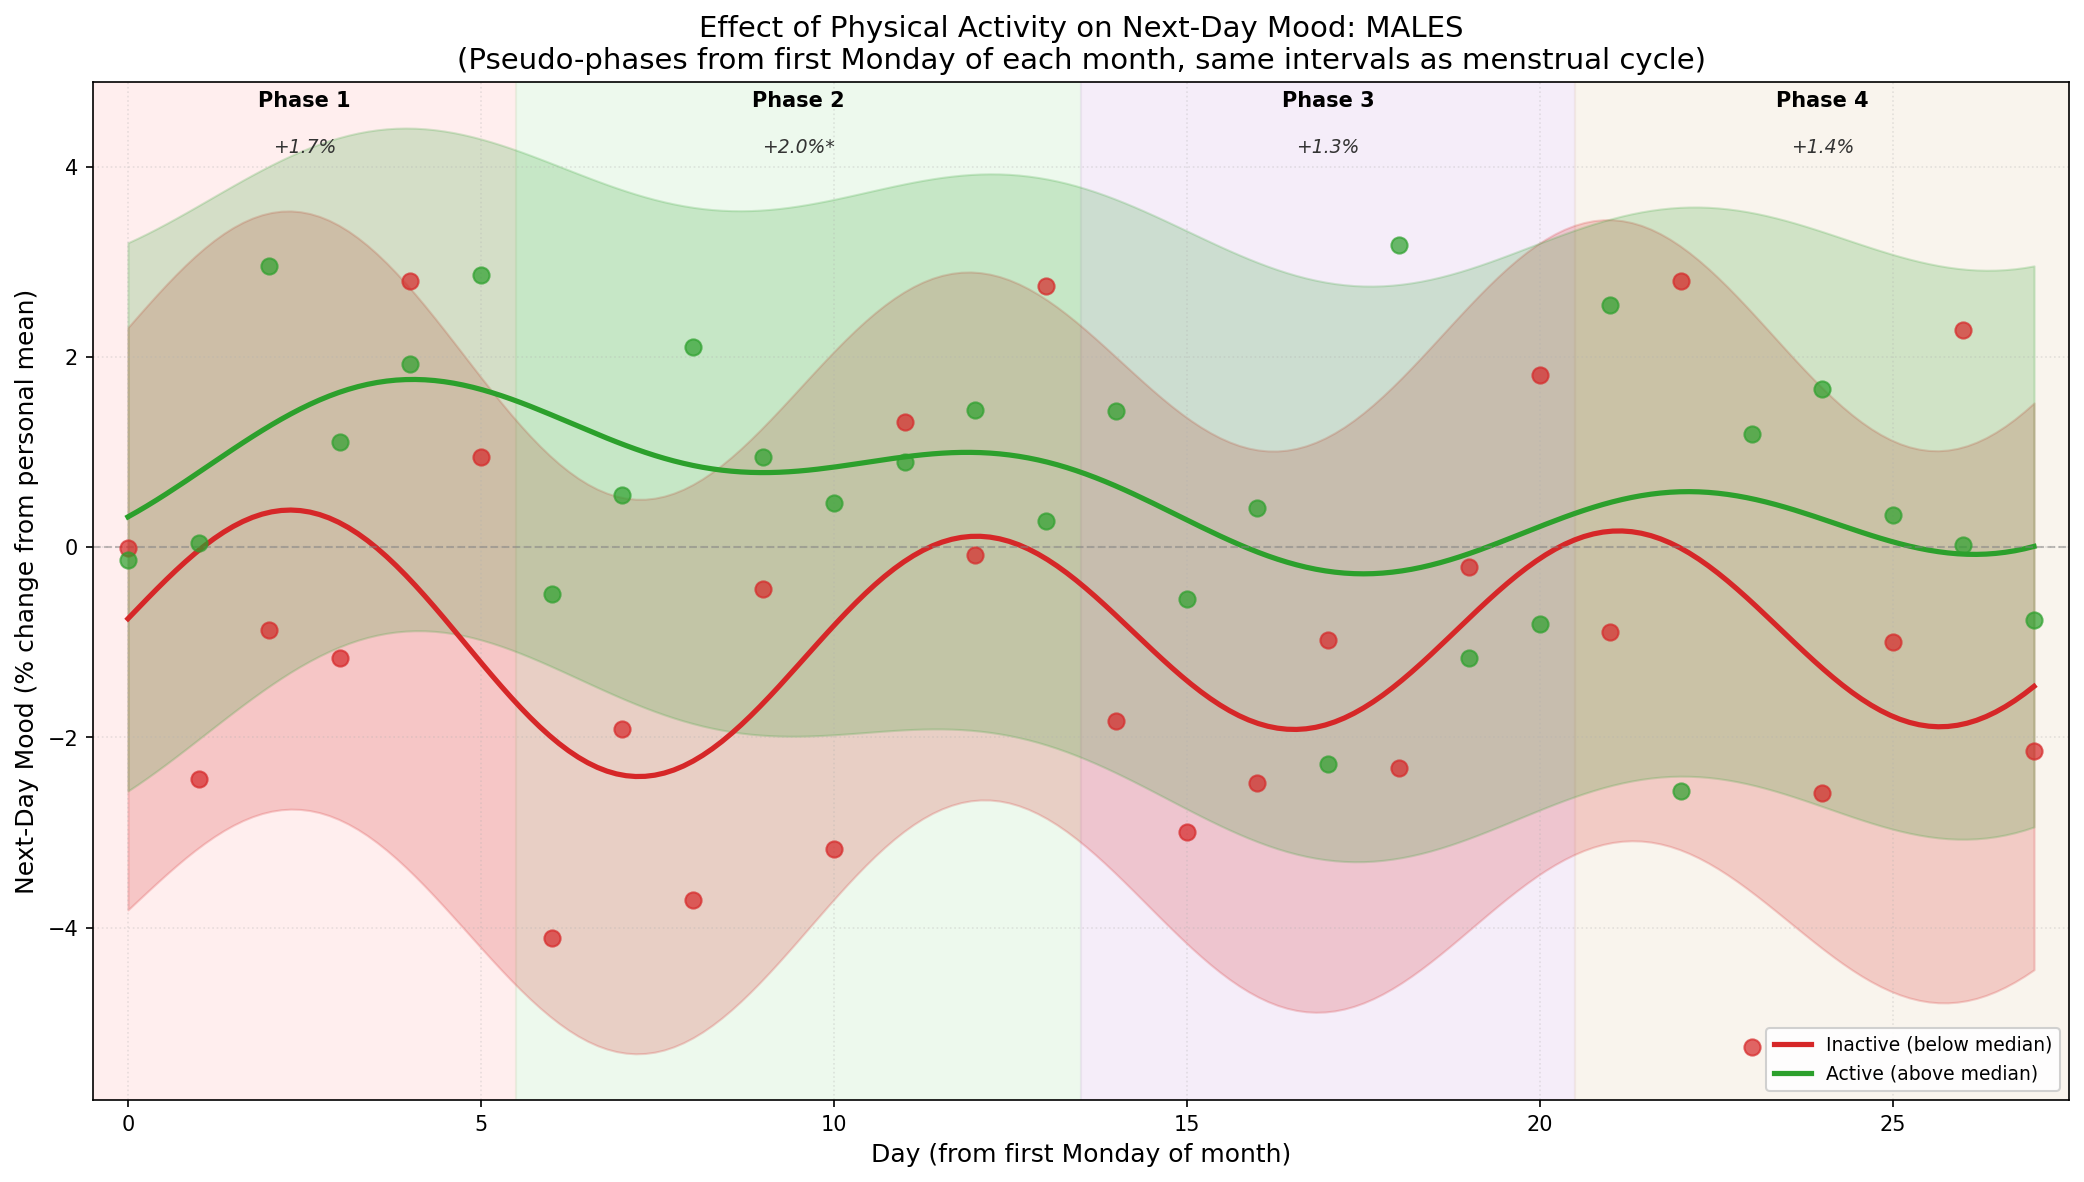
\includegraphics[width=\textwidth]{mood_by_pseudo_cycle_day_males.png}
\fbox{\parbox{0.9\textwidth}{\centering\vspace{3cm}\textbf{Figure 2: Men}\\ Insert mood\_by\_pseudo\_cycle\_day\_males.png\vspace{3cm}}}
\caption{Next-day mood by pseudo-cycle day and activity status in men. Points represent daily means; lines show Fourier-smoothed trajectories with 90\% confidence bands. Background shading indicates pseudo-phases anchored to the first Monday of each month. In contrast to women, the gap between active and inactive days remains relatively constant across all phases.}
\label{fig:men}
\end{figure}

% ============================================
% TABLE 2
% ============================================
\begin{table}[htbp]
\centering
\caption{Phase-specific effects of physical activity on next-day mood}
\label{tab:results}
\begin{tabular}{lcccc}
\toprule
 & \multicolumn{2}{c}{\textbf{Women (n=138)}} & \multicolumn{2}{c}{\textbf{Men (n=966)}} \\
\cmidrule(lr){2-3} \cmidrule(lr){4-5}
\textbf{Phase} & \textbf{Effect (95\% CI)} & \textbf{P value} & \textbf{Effect (95\% CI)} & \textbf{P value} \\
\midrule
Menstruation / Phase 1 & 3.5\% (0.2 to 6.8) & 0.036 & 1.7\% ($-$0.4 to 3.7) & 0.11 \\
Follicular / Phase 2 & 7.6\% (4.6 to 10.7) & $<$0.001 & 2.0\% (0.3 to 3.8) & 0.02 \\
Early luteal / Phase 3 & 3.5\% (0.1 to 6.9) & 0.044 & 1.3\% ($-$0.5 to 3.2) & 0.16 \\
Late luteal / Phase 4 & 0.8\% ($-$2.6 to 4.3) & 0.64 & 1.4\% ($-$0.5 to 3.3) & 0.16 \\
\midrule
\textbf{Heterogeneity test} & $\chi^2$=22.52 & $<$0.0001 & $\chi^2$=7.08 & 0.07 \\
\bottomrule
\end{tabular}
\vspace{0.5em}

\footnotesize
Effects represent percentage change in next-day mood (relative to personal mean) comparing days above versus below personal median activity. Positive values indicate better mood following more active days. CI=confidence interval.
\end{table}

% ============================================
% DISCUSSION
% ============================================
\section*{Discussion}

\subsection*{Principal Findings}

In this observational study of 138 women with menstrual cycle data and 966 men, we found that physical activity was associated with better next-day mood in both sexes. In women, however, this association varied substantially by menstrual cycle phase. The strongest effect occurred during the follicular phase (7.6\% mood improvement), while no significant association was observed during the late luteal phase (0.8\%). Men showed no such phase variation, suggesting the heterogeneity in women reflects menstrual cycle physiology rather than calendar-related confounding.

\subsection*{Comparison with Existing Literature}

% - Consistent with studies showing exercise improves mood generally
% - Extends literature by demonstrating cycle phase as effect modifier
% - Follicular phase findings align with known hormonal profiles:
%   - Rising oestrogen may enhance neuroplasticity and reward sensitivity
%   - Higher energy availability during follicular phase
% - Late luteal null finding aligns with PMS/PMDD literature:
%   - Reduced serotonergic function
%   - May represent period of blunted response to positive stimuli
% - Limited prior work on activity-mood-cycle interaction to compare

\subsection*{Strengths and Limitations}

This study has several strengths. The repeated daily measures within individuals allowed us to use a within-person design, with each participant serving as their own control. The prospective assessment of next-day mood reduces the possibility of reverse causation. The within-person median split for activity classification accounts for individual differences in baseline activity levels. The male control group provides evidence against calendar-related confounding as an explanation for the observed phase heterogeneity in women.

The study also has limitations. Menstrual cycle dates were self-reported without hormonal confirmation, and cycle phases were estimated from period dates rather than ovulation testing. Users of health tracking applications may not be representative of the general population. The observational design precludes causal inference, and we cannot exclude confounding by factors such as sleep, stress, or social activity. The mood measure was a single item from the application rather than a validated scale.

\subsection*{Implications for Practice and Research}

% - Activity promotion may be most effective during follicular/menstruation phases
% - Late luteal phase: activity may still be beneficial but mood effects less pronounced
% - Personalised exercise recommendations could consider cycle phase
% - Cycle-aware mental health interventions warrant investigation

% Future research directions:
% - RCTs with exercise interventions timed to cycle phase
% - Hormonal confirmation of cycle phase
% - Investigation of dose-response relationships by phase
% - Extension to clinical populations (PMDD, depression)
% - Examination of exercise type/intensity interactions

\subsection*{Conclusions}

The association between physical activity and next-day mood is moderated by menstrual cycle phase, with the strongest effect during the follicular phase and no detectable effect during the late luteal phase. The absence of such phase variation in men supports a biological rather than calendar-based explanation. These findings suggest that cycle-aware approaches to physical activity promotion for mental health warrant further investigation.

\end{document}
